\documentclass[11pt,letterpaper]{article}
\usepackage[T1]{fontenc}
\usepackage[utf8]{inputenc}
\usepackage{lmodern,microtype}
\usepackage[margin=0.85in,headheight=15pt,headsep=18pt,footskip=25pt]{geometry}
\usepackage{amsmath,amssymb,mathtools}
\usepackage{booktabs,longtable,array,tabularx}
\usepackage{xcolor,graphicx}
\usepackage{xurl}
\usepackage{tikz}
\usetikzlibrary{arrows.meta,positioning,fit}
\usepackage{enumitem,needspace}
\usepackage{titlesec,fancyhdr,lastpage}
\usepackage{listings}
\usepackage[colorlinks=true,linkcolor=teal,citecolor=teal,urlcolor=teal]{hyperref}
\definecolor{ink}{HTML}{19333C}
\definecolor{teal}{HTML}{176D76}
\definecolor{muted}{HTML}{51616B}
\definecolor{pale}{HTML}{EEF4F5}
\hypersetup{pdftitle={From MOC Verification to an Engine Solver Suite},pdfsubject={Literature-grounded formulation, implementation status, and engine MDO roadmap}}
\pagestyle{fancy}
\fancyhf{}
\fancyhead[L]{\footnotesize\sffamily\color{muted}RaoRocketSim / Solver-suite roadmap}
\fancyhead[R]{\footnotesize\sffamily\color{muted}21 November 2026}
\fancyfoot[R]{\footnotesize\sffamily\color{muted}\thepage\ / \pageref*{LastPage}}
\renewcommand{\headrulewidth}{0.3pt}
\titleformat{\section}{\Large\sffamily\bfseries\color{ink}}{\thesection}{0.7em}{}
\titleformat{\subsection}{\large\sffamily\bfseries\color{teal}}{\thesubsection}{0.6em}{}
\titleformat{\subsubsection}{\normalsize\sffamily\bfseries\color{ink}}{\thesubsubsection}{0.6em}{}
\setlength{\parindent}{0pt}
\setlength{\parskip}{6pt}
\setlength{\emergencystretch}{2em}
\renewcommand{\arraystretch}{1.15}
\setlist{itemsep=3pt,topsep=4pt,leftmargin=1.6em}
\newcolumntype{P}[1]{>{\raggedright\arraybackslash}p{#1}}
\newcommand{\code}[1]{{\small\path{#1}}}
\newcommand{\current}{\textbf{Current implementation.}\ }
\newcommand{\proposal}{\textbf{Proposed implementation.}\ }
\newcommand{\evidence}{\textbf{Evidence and limits.}\ }
\newcommand{\dd}{\mathrm{d}}
\newcommand{\Rt}{R_t}
\newcommand{\Ree}{R_e}
\lstset{basicstyle=\ttfamily\footnotesize,breaklines=true,columns=fullflexible,keepspaces=true,showstringspaces=false,backgroundcolor=\color{pale},frame=none,xleftmargin=6pt,xrightmargin=6pt}
\numberwithin{equation}{section}
\begin{document}
\begin{titlepage}
\vspace*{0.8cm}
{\Huge\sffamily\bfseries\color{ink}From MOC Verification\\[0.15cm]to an Engine Solver Suite\par}
\vspace{0.8cm}
{\Large\sffamily\color{teal}Formulation, implementation status,\\and an MDO integration roadmap\par}
\vspace{0.8cm}
21 November 2026\par
\vspace{1cm}
\textbf{Scope.} Thermodynamically consistent variable-gas flow, shock fitting,
viscous and separated-flow prediction, and a general differentiable
forward-wall characteristic net.
\vspace{0.4cm}
\textbf{Principal finding.} None of the four requested capabilities is complete
as an integrated MOC extension. Substantial reusable components already exist.
The largest engine-integration gap is that the current MDO closes thrust and
throat size with Q1D performance before requesting contour geometry.
\vfill
This is a research and implementation-planning study. It records current code
paths, original-source findings, proposed formulations, dependencies, and
validation requirements. It introduces no new flow solver or default dispatch.
Numerical verification, model applicability, and physical validation are
reported separately.
\end{titlepage}
\tableofcontents
\clearpage
\section{What is implemented, and what remains}
\label{sec:status}

The requested destination is a solver suite that can supply credible nozzle
flow, performance, wall loading and sensitivities to the engine optimizer.
This requires an explicit operating domain and a shared physical state. A
successful MOC design calculation is one component of that suite.

\textbf{Completion count: zero of four at the requested integrated-MOC scope.}
Three areas have reusable numerical or modeling foundations. Shock fitting
has relevant local literature but no identified implemented fitted-shock
path. This count does not erase the functionality of the existing Q1D,
empirical-screening or JAX modules.

\begin{longtable}{@{}P{0.20\linewidth}P{0.36\linewidth}P{0.36\linewidth}@{}}
\toprule
\textbf{Requested capability} & \textbf{What exists} & \textbf{What is still required}\\\midrule
\endhead
Consistent variable-gas MOC &
Frozen-composition, variable-\(c_p\) Q1D expansion; property provenance,
bounded interpolation, enthalpy/entropy integration and sonic closure.
CEA chamber-property surfaces also exist. &
Consistent 2D characteristic equations, gas-dependent starting data,
node state and fluxes; separate equilibrium and finite-rate formulations.
Existing MOC remains calorically perfect.\\
Shock fitting &
Fold/coalescence detection and separation screens identify limitations.
They do not construct a shock. &
Unknown shock geometry, conservative jumps, downstream compatibility,
entropy/composition transport and treatment of subsonic regions.\\
Viscous/separation prediction &
Bartz-based thermal tools, a displacement screening estimate, four empirical
FSS-onset criteria, and an MDO separation margin. &
An integral or resolved nozzle boundary layer coupled to the core,
verified displacement/heat/friction effects, and a defined separated-flow
model. RSS, hysteresis and side loads are not supplied by the screens.\\
General differentiable forward-wall net &
NumPy bounded forward analysis; differentiable throat-arc kernel;
differentiable selected residuals and fixed-state partials. &
Full wall/axis/reflection/start-line/exit dependence, topology-valid
derivatives and total engine sensitivities.\\
\bottomrule
\end{longtable}

The implementation assessment is based on current source and call-path
inspection, with hashes in \code{implementation_inventory.json}. It is not
a new numerical qualification run. Previously completed MOC evidence is
used only where its recorded source hashes still match.

\subsection{What the recent MOC result establishes}
The documented constant-\(\gamma\), inviscid Nozzle-B model passes its
internal gates and a 32/48-to-48/64-point physical-coordinate refinement
comparison. The maximum angle difference is \(0.0228912^\circ\), minimum
field coverage \(0.950270\), and maximum Mach difference \(0.00080366\).
The accepted profile uses exact D/E attachment, explicit kernel capacity
and accurate seed controls. The complete pair took approximately
1,498 seconds; the added refined solve alone took approximately 1,213 seconds.
These are measured costs for that experiment, not representative timing
statistics for the whole solver.

That result demonstrates a usable bounded numerical configuration. It
does not establish variable-gas physics, a fitted shock, viscous interaction,
total wall-design derivatives, or a domain-wide default. The published
Rao example also uses different throat/start-line assumptions. Its
constant-gas variational conditions cannot simply be reused as a proof of
optimality for a reacting or viscous design \cite[PDF pp.~2--5]{rao1958}.

\subsection{Three different problems need separate interfaces}
\begin{enumerate}
\item \textbf{Forward analysis:} prescribe a physical wall, inlet state and
back pressure; determine flow, loads and performance.
\item \textbf{Inverse or variational design:} prescribe performance or
boundary conditions and determine a wall or control surface. The existing
Rao construction belongs here.
\item \textbf{Engine MDO:} vary chamber, geometry, cooling, feed and hardware
variables while closing the coupled engine state and its constraints.
\end{enumerate}
The optimizer needs the derivative of its actual analysis and state closure.
A gradient of an already optimized Rao control surface with respect to
independent solved nodal values is a different object.

\section{Current architecture and the default-solver problem}
\label{sec:architecture}
\subsection{The important live code paths}
\begin{longtable}{@{}P{0.34\linewidth}P{0.58\linewidth}@{}}
\toprule\textbf{Code location} & \textbf{Observed role}\\\midrule
\endhead
\code{raosim/rao_variational.py:solve_rao_bvp} &
Constant-gas control-surface BVP, backward reconstruction, independent
mesh gates and reliability reporting.\\
\code{raosim/moc_bounded.py:march_bounded_net} &
Host forward net with wall/axis handling, physical-strip diagnostics and
explicit incomplete/fold outcomes.\\
\code{raosim/frozen_flow.py:FrozenIdealGasTable} &
Fixed-composition thermally perfect property law and Q1D reference
expansion. Result scope explicitly excludes MOC/Rao characteristics.\\
\code{raosim/physics.py:boundary_layer_displacement} &
Screening estimate labeled repository heuristic, without an established
nozzle validity range; not an integral boundary-layer solve.\\
\code{raosim/separation.py:check_separation} &
FSS-onset screening from Q1D area-station states, or separate frozen Q1D
states; RSS remains unavailable.\\
\code{raosim/jax/moc_kernel.py} &
Padded throat-arc kernel; no general differentiable bounded-wall solver
or complete differentiable starting-line construction.\\
\code{raosim/jax/sensitivities.py} &
Fixed-state control-surface derivatives and explicit parameter partials;
total design and bell-wall dependencies remain deferred.\\
\code{raosim/mdo/nozzle.py:resolve_contour_provider} &
Only the analytic TOP/B\'ezier provider is registered. The typed provider
outcome supports explicit availability/infeasibility.\\
\code{raosim/mdo/contour_validation.py} &
Postsolve comparison against a variational result; it does not replace
the optimizer's inner-loop geometry or thrust law.\\
\bottomrule
\end{longtable}

\subsection{Geometry substitution alone does not change engine aerodynamics}
The current \code{engine_residual} in \code{raosim/mdo/engine.py}
evaluates chamber surfaces and closes the scaled throat radius and mass
flow using
\begin{align}
R_1 &=
\frac{F_{\mathrm{req}}-\eta_{CF}C_{F,\mathrm{1D}}P_c\pi \Rt^2}
     {F_{\mathrm{req}}},\\
R_2 &=
\frac{\dot m-P_c\pi\Rt^2/(\eta_{c^*}c^*_{\mathrm{ideal}})}
     {\dot m_{\mathrm{ref}}}.
\end{align}
These are a transcription of the present software closure, not a proposed
general-gas formula. In \code{solve_engine}, ideal \(C_F\), exit Mach,
exit pressure and separation margin are computed before
\code{evaluate_contour} supplies the cooling/mass grid.

Consequently, registering an MOC geometry provider alone can change wall
geometry, cooling and mass while thrust, throat size and their sensitivities
continue to use the older Q1D performance model. A default transition must
update the coupled aerodynamic state contract and engine residual.

\begin{figure}[htbp]
\centering
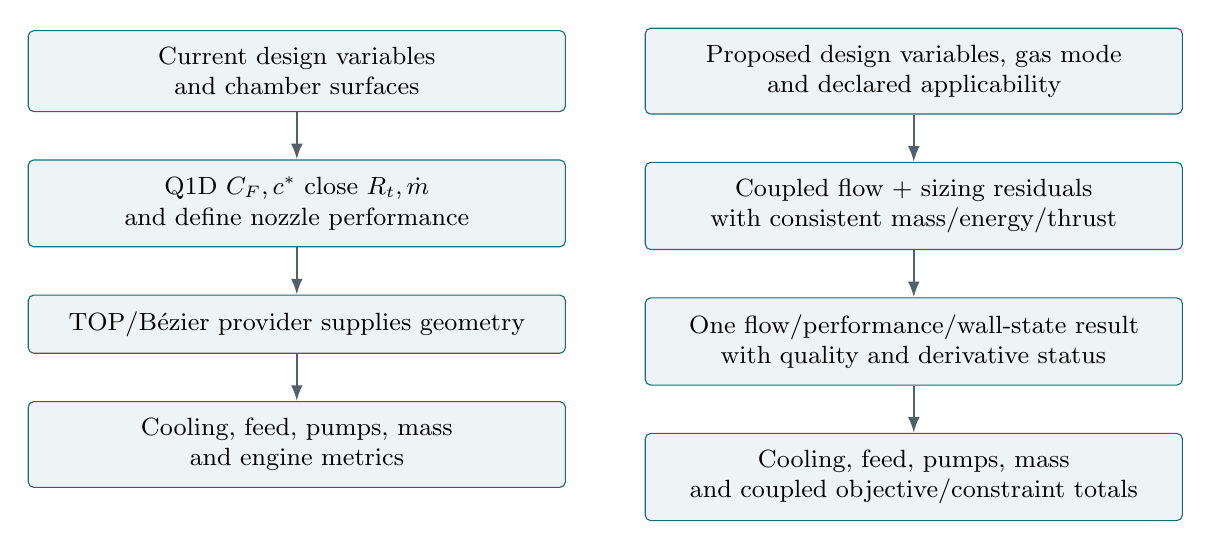
\begin{tikzpicture}[
box/.style={draw=teal,rounded corners=2pt,fill=pale,text width=6.4cm,
align=center,font=\small,inner sep=6pt},
arr/.style={-{Latex[length=2mm]},thick,draw=muted},
node distance=6mm]
\node[box] (a) {Current design variables and chamber surfaces};
\node[box,below=of a] (b) {Q1D \(C_F,c^*\) close \(\Rt,\dot m\)\\and define nozzle performance};
\node[box,below=of b] (c) {TOP/B\'ezier provider supplies geometry};
\node[box,below=of c] (d) {Cooling, feed, pumps, mass\\and engine metrics};
\node[box,right=10mm of a] (e) {Proposed design variables, gas mode\\and declared applicability};
\node[box,below=of e] (f) {Coupled flow + sizing residuals\\with consistent mass/energy/thrust};
\node[box,below=of f] (g) {One flow/performance/wall-state result\\with quality and derivative status};
\node[box,below=of g] (h) {Cooling, feed, pumps, mass\\and coupled objective/constraint totals};
\draw[arr] (a)--(b); \draw[arr] (b)--(c); \draw[arr] (c)--(d);
\draw[arr] (e)--(f); \draw[arr] (f)--(g); \draw[arr] (g)--(h);
\end{tikzpicture}
\caption{Current dependency order and proposed integration target.
The right-hand structure is a design proposal; it is not the present MDO implementation.}
\end{figure}

\subsection{Three existing \(c^*\) conventions must be reconciled}
\begin{longtable}{@{}P{0.30\linewidth}P{0.32\linewidth}P{0.30\linewidth}@{}}
\toprule\textbf{Path} & \textbf{Current computation} & \textbf{Integration implication}\\\midrule
\endhead
Host \code{cea.cea_propellant} &
Obtains RocketCEA \code{get_Cstar}. &
Chemical mode, database and station conventions must be preserved.\\
Host \code{frozen_flow} &
Computes \(c^*=p_0/G_*\) from its integrated variable-\(c_p\) sonic state. &
A physically distinct fixed-composition Q1D model.\\
MDO \code{ChamberSurfaces.c_star_ideal} &
Uses the calorically perfect analytic law evaluated with interpolated
\(\gamma,T_c,R\). The sampled CEA fields are these three quantities,
not \(c^*\) or \(G_*\). &
Sampling chamber properties does not automatically import the full
CEA or variable-property sonic closure into MDO.\\
\bottomrule
\end{longtable}

\subsection{A proposed shared flow-result contract}
\proposal Introduce one result consumed by sizing, cooling, structural
screens and reporting. It should include the physical wall and effective
core geometry; inlet and local gas-mode identifiers; mass flux; thrust and
its control-volume basis; wall-edge \(p,T,\rho,V,M\), composition and
transport properties; shock/boundary-layer state where applicable; and
reference units and station conventions.

Availability, physical-domain status, conservation residuals, resolution
evidence and derivative validity must be separate fields. A finite,
fixed-shape array used to carry an infeasible candidate through JAX is
not a valid flow field. The present typed contour-provider behavior is
useful infrastructure for this distinction.

No explicit fallback should be hidden inside a higher-fidelity result.
Lower-fidelity analysis can be selected or used to initialize another
solver, with the executed model recorded in the result and optimizer
history.

\section{Thermodynamically consistent variable-gas formulations}
\label{sec:thermo}
\subsection{The gas model is a constitutive system}
The current MOC uses constant-\(\gamma\) Prandtl--Meyer functions,
isentropic power laws, characteristic coefficients and transonic starting
data. Replacing \(\gamma\) at individual stations leaves these ingredients
mathematically inconsistent unless the equations are rederived for the
selected thermodynamic regime. Anderson explicitly distinguishes an
effective \(\gamma\) fitted to one relation from an exact representation
of all the other relations \cite[\S17.6, PDF pp.~684--685]{anderson}.

\begin{longtable}{@{}P{0.20\linewidth}P{0.35\linewidth}P{0.37\linewidth}@{}}
\toprule\textbf{Regime} & \textbf{Closure} & \textbf{MOC implication}\\\midrule
\endhead
Calorically perfect &
Fixed composition and constant \(c_p,c_v,R,\gamma\). &
Present branch; retain as the limiting-case regression.\\
Thermally perfect, frozen composition &
Fixed species mass fractions \(Y_i\), but \(c_p(T)\) varies.
A single temperature and internal-mode equilibrium are explicit choices. &
First practical variable-property branch; use a consistent EOS,
enthalpy, entropy and frozen acoustic speed.\\
Chemical equilibrium &
Composition follows local equilibrium subject to element conservation. &
Requires constrained equilibrium derivatives and the appropriate
equilibrium acoustic closure. A frozen \(c_p(T)\) table is insufficient.\\
Finite-rate nonequilibrium &
Composition and possibly internal-mode energies evolve along flow history. &
Adds species/relaxation transport and stiffness. Entropy need not be
constant in inviscid adiabatic expansion.\\
\bottomrule
\end{longtable}

These distinctions follow the original thermodynamics discussion, not
software naming conventions \cite[\S\S17.4--17.9, PDF pp.~675--689]{anderson}.
An equilibrium/frozen label must specify what is frozen, at which station,
and with which composition, internal-mode and thermodynamic data.

\subsection{First target: fixed-composition thermally perfect gas}
For a single-phase ideal mixture with fixed \(Y_i\),
\begin{align}
R &= \sum_iY_i R_i, & p&=\rho RT,\\
c_p(T)&=\sum_iY_i c_{p,i}(T),&
c_v(T)&=c_p(T)-R,\\
h(T)-h(T_{\mathrm{ref}})
&=\int_{T_{\mathrm{ref}}}^{T}c_p(\tau)\,\dd\tau,\\
s(T,p)-s(T_{\mathrm{ref}},p_{\mathrm{ref}})
&=\int_{T_{\mathrm{ref}}}^{T}\frac{c_p(\tau)}{\tau}\,\dd\tau
-R\ln\!\left(\frac{p}{p_{\mathrm{ref}}}\right).
\end{align}
The original text gives the thermally perfect entropy integral and
enthalpy identities explicitly \cite[\S1.4.5, PDF pp.~40--44,
Eqs.~1.18, 1.20, 1.32--1.35; \S17.4, PDF p.~678]{anderson}.
The frozen small-disturbance sound speed is
\begin{equation}
a_f^2=\left(\frac{\partial p}{\partial\rho}\right)_{s,Y}
=\gamma_f(T)RT,\qquad
\gamma_f=\frac{c_{p,f}}{c_{v,f}},
\end{equation}
under these assumptions \cite[\S17.5, PDF p.~682, Eq.~17.36]{anderson}.
This acoustic definition, rather than an arbitrary chamber \(\gamma\),
sets local \(M=V/a_f\) and the Mach angle.

\current \code{FrozenIdealGasTable} already integrates enthalpy and
standard entropy from its bounded \(c_p(T)\) representation.
\code{solve_frozen_nozzle_expansion} closes a sonic throat and Q1D area
stations. Its result explicitly excludes MOC/Rao characteristics and
equilibrium chemistry. Reuse of this module should preserve its data
identity, composition/freeze basis, domain checks and conservation tests.

\proposal Put the property calculation behind a state contract
\[
\mathcal{G}:\quad
(p,T,Y;\hbox{gas mode, data identity})
\longmapsto
(\rho,h,s,a^2,c_p,\hbox{required partials},\hbox{validity}).
\]
Each requested derivative must use the same composition and equilibrium
constraints as the state. Store units, reference enthalpy convention,
species set, property source/version/hash and admissible domain with
the model. Include viscosity and conductivity through a separately
identified transport closure; an EOS alone does not provide them.

For smooth optimization, interpolation regularity also matters. The
present piecewise-linear \(c_p\) law gives consistent integrals, but
derivatives can change at property-grid knots. Any smoother replacement
must preserve \(h_T=c_p\), \(s_T|_p=c_p/T\), positivity and
\(c_p-c_v=R\); independently fitting inconsistent \(h,s,c_p\) surfaces
would defeat the purpose.

\subsection{Generalize the compatibility variables, not only the coefficient}
For smooth isentropic turning, the velocity differential
\begin{equation}
\dd\mathcal{N}=\sqrt{M^2-1}\,\frac{\dd V}{V}
\label{eq:turning}
\end{equation}
defines a path-dependent turning increment before the calorically perfect
specialization. Anderson's Eq.~4.35 gives the corresponding turning
differential; Eqs.~4.39--4.44 specialize and integrate
it for the closed Prandtl--Meyer function
\cite[\S4.14, PDF pp.~186--187]{anderson}.

In the smooth, steady, adiabatic, irrotational/homentropic axisymmetric
case, the velocity-form compatibility retains the geometric source:
\begin{align}
C^+:\quad \dd\theta-\dd\mathcal{N}
&=-\frac{\sin\theta}{Mr}\,\dd\ell,
&\frac{\dd r}{\dd x}&=\tan(\theta+\mu),\\
C^-:\quad \dd\theta+\dd\mathcal{N}
&=+\frac{\sin\theta}{Mr}\,\dd\ell,
&\frac{\dd r}{\dd x}&=\tan(\theta-\mu).
\end{align}
Here \(\ell\) is characteristic arclength oriented downstream, distinct
from thermodynamic entropy \(s\), and \(\mu=\sin^{-1}(1/M)\).
The displayed source form applies for \(r>0\); the axis requires a
separately regularized symmetry limit. Backward reconstruction must
retain the same signed orientation convention.
The original axisymmetric derivation uses \(dp=-\rho V\,dV\) and the
isentropic acoustic derivative before introducing the perfect-gas
Prandtl--Meyer function
\cite[\S11.4, PDF p.~408; \S11.8, PDF pp.~420--422,
especially Eq.~11.51]{anderson}.

For the first frozen-property target, recover local \(T,p,\rho,a\) from
\(h_0=h(T)+V^2/2\), the chosen isentrope and EOS. A turning integral or
its differential then depends on that thermodynamic path. It is not the
old universal \(\nu(M;\gamma)\) with a varying argument inserted into it.
Across streamline entropy differences, finite-rate chemistry,
independently varying composition, heat addition or shocks, additional
transport and compatibility terms are required. Smooth homentropic
equilibrium flow can still use a consistently closed EOS in this framework.
Equations above do not claim to supply that larger system.

\subsection{Starting data, sonic closure and conservation}
The transonic starting line must be consistent with the chosen gas law
and throat curvature. A variable-property downstream solver started from
an unverified constant-gas KL expansion is a mixed formulation. The
original KL coefficient table remains unavailable in the prior audit;
this is a separate source gap to resolve or avoid with a verified
alternative initializer.

The first milestone should therefore include the Q1D sonic state,
throat mass flux, a source-grounded transonic/near-sonic initializer and
convergence away from any numerical supersonic offset. Track the reference
state used to define \(c^*\), Mach and mass flow. Require independent
conservation checks rather than rescaling the starting line to an ideal
one-dimensional mass flow by construction.

For nonequilibrium flow, the sonic location is not in general guaranteed
to coincide with the geometric throat. The original text also makes
clear that finite-rate irreversibility breaks isentropy in an otherwise
inviscid adiabatic nozzle \cite[\S17.11, PDF p.~704]{anderson}. The
current frozen sonic-root assumptions cannot be carried into that
branch without a new derivation.

\subsection{Equilibrium and finite-rate branches}
At equilibrium, composition derivatives contribute to heat capacities:
\begin{equation}
c_{p,\mathrm{eq}}
=\sum_iY_i c_{p,i}
+\sum_i h_i\left(\frac{\partial Y_i}{\partial T}\right)_p .
\end{equation}
The source separately defines frozen and equilibrium heat capacities
\cite[PDF p.~678, Eqs.~17.20--17.25]{anderson}.
Formation-energy conventions matter when \(Y_i\) changes. A chamber
property table in \((P_c,\mathrm{O/F})\) is not a complete
local equilibrium EOS in the nozzle.

For an equilibrium EOS expressed in \((\rho,T)\), the following total
differential is a useful proposed implementation check:
\begin{equation}
a_{\mathrm{eq}}^2
=p_\rho|_T-p_T|_\rho\frac{s_\rho|_T}{s_T|_\rho}.
\end{equation}
This follows by imposing \(\dd s=0\) on a differentiable single-phase
equilibrium branch with fixed elemental inventory and \(s_T|_\rho\ne0\).
It is an identity to test against the thermodynamic backend,
not a replacement for computing consistent equilibrium derivatives.
Anderson's more explicit sound-speed expression includes the
non-perfect-gas derivative corrections \cite[PDF p.~682, Eq.~17.35]{anderson}.

A single-temperature finite-rate ideal-mixture branch would additionally
solve, under its declared inviscid assumptions,
\begin{equation}
\frac{D Y_i}{Dt}=\frac{\dot\omega_i}{\rho},\qquad
\sum_iY_i=1,\qquad \sum_i\dot\omega_i=0.
\end{equation}
The production units are \(\mathrm{kg\,m^{-3}\,s^{-1}}\).
Species transport is source-grounded
\cite[PDF p.~687, Eq.~17.42]{anderson}. A reacting
characteristic intersection needs streamline history as well as its
two acoustic parents. The local Young thesis constructs that third
streamline foot explicitly \cite[PDF pp.~91--96]{young}.

The absolute mixture enthalpy must include formation contributions
consistently. Chemical energy cannot also be added as a second external
heat-release term if already present in that enthalpy. Finite-rate
species and internal-mode relaxation can introduce stiff source
integration and additional sound/characteristic conventions.

\subsection{A source discrepancy that blocks direct finite-rate transcription}
Independent checks of the original Young thesis found unresolved
differences between its earlier EOS/absolute-enthalpy definitions and
the printed chemical-source expression. PDF pp.~87--89 define
\(R=\sum_iY_iR_i\), mass production and \(h_i+h_i^\circ\), whereas
Eqs.~4.22--4.23 print a common mixture \(R\) and
\(h_i-h_i^\circ\). A separate units check found a discrepancy between
Eq.~4.49 and the subsequent coefficient forms on PDF pp.~93--94.

These are recorded as source inconsistencies and independently derived
candidates in \code{source_discrepancies.json}, not as an established
published erratum. Young remains useful evidence for the coupled
characteristic/streamline architecture. Its printed source coefficients
are not implementation-ready until rederived and corroborated against
the original governing formulation. This blocks that transcription,
not the earlier fixed-composition thermally perfect milestone.

\section{Shock fitting and the postshock flow}
\label{sec:shock}
\subsection{A fitted shock is an unknown boundary}
Shock fitting represents a discontinuity explicitly and solves for its
position/orientation together with the flow on each side. Shock capturing
instead represents the jump through a discretized conservation-law field.
The original MOC treatment matches downstream characteristic information
to the shock relations \cite[\S11.5.3, PDF p.~411;
\S11.15, PDF p.~438]{anderson}.

The current code's cell-fold or coalescence detection is a useful refusal
mechanism for its smooth march. A fold alone does not select an admissible
shock, establish its location, or prove that a physical shock rather than
under-resolution caused the failure. No fitted-shock solve was located in
the current \code{raosim} paths.

\subsection{Conservation is necessary but does not locate the front}
For a locally stationary adiabatic inviscid shock without external work, with normal directed from
upstream 1 to downstream 2 and nonzero normal mass flux \(j\),
\begin{align}
j&=\rho_1V_{n1}=\rho_2V_{n2},\\
p_1+\rho_1V_{n1}^2&=p_2+\rho_2V_{n2}^2,\\
V_{t2}&=V_{t1},\\
h_1+\tfrac12|\mathbf V_1|^2&=
h_2+\tfrac12|\mathbf V_2|^2 .
\label{eq:RH}
\end{align}
These are local conservation relations, with tangential continuity for
the stated inviscid stationary setting. They are not restricted to a
calorically perfect gas
\cite[\S3.6, PDF p.~104, Eqs.~3.38--3.40;
\S4.3, PDF pp.~150--151, Eqs.~4.3--4.6]{anderson}.

They must be closed using the same EOS, enthalpy/composition convention
and acoustic mode as the rest of the flow. Upstream \(p,T,\mathbf V,Y\),
the front normal, and an entropy-admissible compressive root are needed.
The trivial unshocked root must be excluded. For a general reacting EOS,
an upstream Mach number alone does not specify the dimensional state
\cite[\S17.2, PDF pp.~665--668]{anderson}.

Front geometry is determined by additional characteristic, wall,
symmetry-axis and downstream-pressure conditions. The familiar
\(\theta\)--\(\beta\)--\(M\) relation is a calorically perfect limiting
test, not a general-gas closure with locally substituted \(\gamma\).
Weak/strong roots, attached-front limits and pressure-dependent branch
selection must remain explicit \cite[PDF pp.~152--154]{anderson}.

\subsection{Curved shocks require rotational transport}
A curved front generally produces different entropy jumps between
streamlines when its shock strength varies.
The postshock state therefore needs more information than the current
smooth isentropic C+/C- invariants. Anderson's rotational MOC carries
streamline entropy and total enthalpy in addition to the Mach-line data,
including an interpolated streamline foot
\cite[\S11.9, PDF pp.~423--424]{anderson}.

\proposal Represent separate flow regions and an explicit shock-front
mesh. Shock nodes should reference their upstream sampling location,
front normal, jump result and downstream characteristic parents.
Transport entropy/enthalpy or equivalent conservative thermodynamic
information into the downstream rotational unit processes. Include
composition and relaxation history for a reacting branch.

Conserve total enthalpy rather than assuming unchanged total temperature
for all gas models. Likewise, the calorically perfect relation between
entropy rise and stagnation-pressure loss cannot be transferred without
qualification to changing-composition states
\cite[PDF p.~109, Eqs.~3.61--3.63]{anderson}.

\subsection{Frozen fronts, reacting relaxation and mixed-type limits}
Frozen jump conditions followed by finite-rate downstream relaxation
describe a different model from an equilibrium jump. The source
distinguishes the very short shock-front scale from chemical relaxation
downstream \cite[\S17.10, PDF pp.~690--691]{anderson}.
The selected model should name these assumptions and their reference
evidence, rather than silently relaxing to a preferred equilibrium state.

Steady supersonic MOC requires a locally supersonic marching region.
A normal shock or sufficiently strong oblique shock can create a
subsonic downstream region. Separation also introduces recirculation and
viscous interaction. These regions require a coupled mixed-type or
viscous method with the appropriate boundary conditions. A hyperbolic
characteristic march alone cannot supply that solution
\cite[PDF p.~411]{anderson}\cite[PDF pp.~4--5]{pns}.

The first fitted-shock milestone should therefore be deliberately
restricted: a specified stationary topology and gas mode, with an
admissible supersonic downstream region where the chosen MOC applies.
Shock--wall/axis intersections, shock interactions and slip lines are
additional topology milestones. General off-design back-pressure
analysis needs an explicit subsonic/separated-flow route.

\section{Viscous interaction, heat transfer and separation}
\label{sec:viscous}
\subsection{Attached boundary layers are a separate flow model}
\current The repository has heat-transfer/cooling models, a
displacement/area-loss screen and empirical separation criteria.
\code{physics.boundary_layer_displacement} labels its nozzle extension
as a heuristic without a located validity range. None evolves a
compressible nozzle boundary layer and iterates its displacement into MOC.

NASA SP-8120 calls for integral momentum and energy boundary-layer
analysis with friction/heat-transfer closures, and for displacement
thickness in performance prediction \cite[PDF p.~27, printed p.~13]{sp8120}.
That passage supplies the modeling requirement and references; it is not
itself a complete axisymmetric closure set ready to transcribe.

\proposal Introduce an attached boundary-layer state with source-selected
definitions for momentum/energy thickness or profiles; edge
\(p_e,\rho_e,U_e,h_e,Y_e\); transition/relaminarization assumptions;
wall temperature/chemistry/roughness; skin friction; heat flux; and
pressure-gradient/axisymmetric terms. Transport and thermal property
models need independent identity and applicability.

A proposed local displacement convention, derived by replacing the
integrated mass deficit with an equivalent edge-state strip and written
in a wall-normal coordinate \(n\), is
\begin{equation}
\delta^*=\int_0^\infty
\left(1-\frac{\rho u}{\rho_eU_e}\right)\,\dd n .
\end{equation}
This is a project definition of the local mass deficit, not a
source-transcribed closure. It is not the complete
axisymmetric integral boundary-layer method or a proposed universal
velocity-profile closure. Those geometry and closure choices remain
implementation dependencies.

\subsection{Preserve the physical wall and distinguish forward from inverse use}
For a prescribed metal wall, displacement reduces the effective core.
In a thin, locally near-axial approximation one may interpret
\begin{equation}
A_{\mathrm{core}}\simeq\pi(r_w-\delta^*)^2.
\end{equation}
This is a proposed geometric interpretation for forward analysis.
The actual implementation must derive the correct local-normal and
axisymmetric projection rather than applying this scalar radial formula
to an arbitrary steep wall.

SP-8120's outward wall correction is an inverse-design compensation:
move the design wall outward to retain a desired inviscid core
\cite[PDF p.~27]{sp8120}. A forward analysis call should not alter the
manufactured wall or export displacement as hardware geometry.
Maintain physical-wall, core-edge and thermal-station coordinates
separately and iterate their consistent coupling.

\subsection{Energy and loss accounting must close with the coolant solution}
Skin friction changes momentum and total-pressure loss. Wall heat loss
changes gas enthalpy, coolant enthalpy and performance. A local heat
correlation used by the cooling module is not a resolved viscous flow field.
A coupled calculation should pass the edge state and wall temperature
between core/BL/thermal models and close a common energy ledger.

The Wang nozzle study explicitly couples species, momentum and total
enthalpy, and compares adiabatic and cooled-wall predictions
\cite[PDF pp.~2, 5, 7]{wang}. Its mechanism and radiation observations
are case-specific; they do not establish a universal mechanism or justify
omitting radiation in every propellant.

When a physical loss is already represented in the flow and exit flux,
do not subtract the same effect again through a drag decrement and a
generic \(\eta_{CF}\). Residual efficiency factors may remain for
explicitly unmodeled losses, with their meaning recorded.

\subsection{Thin attached-layer corrections have an applicability boundary}
Strong acceleration, transition, relaminarization, wall cooling and
low Reynolds number complicate nozzle boundary layers. When displacement
is comparable to the nozzle radius, a separate inviscid core plus small
correction may break down. Streamwise-separated regions also violate the
assumptions of simple downstream viscous marching
\cite[PDF pp.~4--5]{pns}\cite[PDF p.~33]{sp8120}.

No universal displacement ratio or Reynolds cutoff is adopted here.
Source-selected limits and validation-domain decisions must accompany
the model. A residual converging numerically does not establish that
its attached-layer assumptions remain applicable.

\subsection{Separation onset, pattern, reattachment and side loads}
\current \code{separation.py} implements Summerfield, Schilling,
Kalt--Badal and Schmucker onset screens, with explicit FSS-only scope.
The local MDO uses a Schmucker margin. Wall-station inputs are reconstructed
from Q1D area states or the separate frozen expansion; the function does
not consume a resolved MOC pressure/BL field.

The original separation review discusses scatter and the distinction
between shock-interaction pressure rise and recirculation recovery
\cite[\S6.3.1, PDF pp.~51--52]{ostlund}. SP-8120 describes separation
criteria as development guides and calls for full-scale checks of
marginal designs \cite[PDF p.~82]{sp8120}. Existing screening should be
retained with its scope, not relabeled as resolved separated flow.

A broader suite must distinguish:
\begin{itemize}
\item incipient interaction and actual separation location;
\item free shock separation (FSS), restricted shock separation (RSS),
reattachment and recirculation/plateau pressure;
\item steady branch selection versus startup/shutdown history;
\item mean axisymmetric loads versus unsteady asymmetric side loads.
\end{itemize}
For the cited VOLVO S1 case, the source reports different FSS/RSS states
at the same pressure ratio on startup and shutdown, with transitions
near 15 and 12 respectively \cite[\S8.1.1, PDF p.~70]{ostlund}.
These are case observations, not transferable default thresholds.
A memoryless smooth NPR-to-pattern function cannot reproduce both states.

For the pressure contribution of a circumferentially symmetric solution,
\[
\mathbf F_\perp=\int_{\mathrm{wall}}p\,\mathbf n_\perp\,\dd A=\mathbf0
\]
by symmetry; symmetric viscous tractions also cancel laterally.
A steady axisymmetric MOC/BL result therefore cannot itself
provide a directional side-load time history. Side-load prediction needs
an independently calibrated statistical model or asymmetric unsteady
viscous simulation and structural/measurement transfer information
\cite[PDF pp.~70, 78--82]{ostlund}\cite[PDF p.~6]{frey}.

\proposal First connect source-appropriate onset screens to resolved wall
edge states while retaining their calibrated Mach, geometry and thermal
scope. Then develop a separately identified shock/BL interaction and
separated mixed-type model. RSS and side-load products require their own
validation, even when offered behind a common user-facing solver suite.

\section{A general differentiable forward-wall net}
\label{sec:ad}
\subsection{Differentiate the solved analysis, including its boundaries}
The requested object is a prescribed-wall flow operator with wall,
inlet/gas, symmetry and exit dependence. It must include the starting
line, every propagated parent, wall intersections/tangency, axis
reflections, post-D/BDE regions where used, and the final momentum,
pressure, mass and energy integrals.

\current The host bounded forward net and JAX throat kernel provide
useful references. The JAX \code{build_start_line} path still raises
\code{NotImplementedError}. The sensitivity API supplies selected
fixed-state partials and explicitly defers total solved-design and
bell-wall derivatives; it refuses the exact-D mode used by the recent
accepted profile. This is not an end-to-end differentiable arbitrary-wall
analysis or a total-gradient API for that profile.

\proposal Reuse the host implementation as a primal oracle within its
established domain, while separating continuous unit-process solves
from discrete topology construction. The first full differentiable
target should be attached, smooth, calorically perfect flow with
matched starting data. Add other physical regimes after this complete
chain is validated.

\subsection{Record the topology and its validity neighborhood}
A proposed topology record should include parent indices, row masks and
widths, raw/special insertions, wall and axis reflection roles, interpolation
brackets, intersection branches, shock-region labels, exit cropping and
termination reasons. Within one accepted topology, solve continuous
unit-process residuals with explicit convergence and conditioning checks.

The presence of \code{stop_gradient} or a fixed-shape mask does not prove
that a discrete decision is irrelevant to the physical derivative.
Changing a wall-intersection bracket, reflection count, active constraint,
shock attachment, separation pattern, mesh topology or property branch
can change the differentiated problem. A physically continuous output
may still have a non-smooth discrete approximation or different one-sided
derivatives.

A practical proposed policy is to diagnose an admissible local topology
neighborhood, use trust-region steps within it, and rebuild/revalidate
when events occur. At an event, mark the ordinary smooth derivative
unavailable or provide explicitly validated one-sided/branch derivatives.
Smoothing a switch is a modeling/numerical approximation whose bias must
be measured; it is not automatically the derivative of the unsmoothed
flow.

\subsection{Root, optimization and iteration derivatives are different}
For a converged square residual
\begin{equation}
F(z,x)=0,\qquad
F_z z_x=-F_x,
\label{eq:IFT}
\end{equation}
implicit sensitivities require a differentiable local residual and
nonsingular state Jacobian. A transposed linear solve gives an adjoint
form for scalar output \(J(z,x)\):
\begin{equation}
F_z^\mathsf{T}\lambda=J_z^\mathsf{T},
\qquad
\frac{\dd J}{\dd x}=J_x-\lambda^\mathsf{T}F_x.
\end{equation}
Blondel et al.\ give the root/optimality-condition framework and discuss
approximate-solve error \cite[\S2.1, PDF pp.~3--4;
\S3, PDF p.~6]{blondel}. These hypotheses are requirements to check for
the chosen MOC system, not properties conferred by using an AD library.

For an overdetermined least-squares calculation with a nonzero final
residual, the stationarity or active-set/KKT system is the relevant
implicit object. For fixed symmetric weights \(W\),
\begin{align}
\phi(z,x)&=\tfrac12r^\mathsf{T}Wr,&
g(z,x)&=J_r^\mathsf{T}Wr=0,\\
g_z&=J_r^\mathsf{T}WJ_r+
\sum_i(Wr)_i\nabla_z^2r_i.
\end{align}
This displayed Hessian follows by differentiating that objective.
Dropping its residual-curvature term is a Gauss--Newton approximation,
not automatically the derivative of the exact optimum. Reduced D/E
parameterizations, design-dependent weights/bounds and stable active
constraints require their full chain rules.

Differentiating a fixed number of nonlinear iterations gives the
derivative of that algorithmic output. It approaches a solved-state
derivative only under additional convergence/regularity conditions.
The existing library supports multiple adjoint strategies, but installed
behavior and the actual differentiated residual must be audited before
selecting one \cite{optimistix}. No present implementation defect in
the library is asserted here.

\subsection{What a meaningful derivative test looks like}
\begin{enumerate}
\item Check the full primal result against the host oracle on the same
wall, gas state, topology and numerical policy.
\item Verify each continuous gas, intersection, wall, axis and exit
operator, including implicit-root contributions.
\item Perform full-output directional Taylor tests:
\[
E(h)=\left|J(x+hv)-J(x)-h\,D J(x)v\right|.
\]
For a smooth sufficiently accurate solve, the first-order remainder
should show the expected second-order regime before roundoff/primal
error dominates. Sweep step sizes; one finite-difference agreement
does not establish a useful error regime.
\item Repeat under physical-grid, property-grid and nonlinear-tolerance
refinement. Primal error must be below the tested signal, and adjoint
residual/conditioning should be recorded.
\item At topology or physical-regime events, compare admissible one-sided
branches rather than treating an across-event centered difference as a
smooth-gradient oracle.
\end{enumerate}
Test wall controls, \(\Rt,R_u,R_d,\epsilon,L\), chamber state and gas
parameters wherever supported. For engine totals include chamber
thermochemistry, composition, starting-line, inner wall temperature,
throat/mass-flow closure and the output's direct parameter dependence.

\subsection{Cost and memory are part of the design}
An adjoint can avoid forming every design-state Jacobian column, but it
does not make the primal analysis free. Padded characteristic histories,
nonlinear correctors, equilibrium/species solves and reverse-mode storage
can all be large. The current throat representation also grows as
rows widen. Measure scaling with actual accepted problem sizes.

Sparse/local residual structure, converged unit-process implicit solves,
checkpointing, branch-consistent warm starts and compiled reuse are
candidate techniques. Cache keys must bind geometry, gas/data identity,
boundary conditions, topology and numerical policy. Reusing a previous
converged root is an initialization strategy; accepting an unconverged
history-dependent result would change the analysis.

The forward-wall operator is a useful priority because it can avoid
solving a fresh inverse contour-optimization problem for each outer wall
candidate. Any cost advantage remains to be demonstrated by profiling.
The recently measured 25-minute pair cannot be assumed suitable for
thousands of nested MDO evaluations.

\section{Effects on full-engine MDO}
\label{sec:mdo}
\subsection{The state closure must use the same aerodynamics as the objective}
\proposal A coupled formulation can collect throat/mass-flow states
\(y=(\Rt,\dot m)\), flow/BL states \(z\), wall/coolant states \(w\), and
design \(x\) into residuals of the form
\begin{align}
R_F&=F_{\mathrm{flow}}(z,w,y,x;p_a)-F_{\mathrm{req}},\\
R_m&=\dot m-A_tG_{*,\mathrm{del}}(y,x;\mathcal G),\\
R_{\mathrm{flow}}&=0,\qquad
R_{\mathrm{BL/thermal}}=0.
\end{align}
This is an architecture proposal. Here \(G_{*,\mathrm{del}}\) is the
mass flux averaged over the declared reference throat area; a
nonuniform throat requires the corresponding mass-flow integral.
The delivered sonic mass-flux model
must declare combustion/loss conventions rather than double-counting
an existing \(c^*\) efficiency. For each regime, performance should come
from a declared consistent control volume with momentum, pressure,
mass and energy accounting.

Whether implemented monolithically or by nested solves, the linearized
coupling must be present in the total derivative. For example,
\begin{equation}
\begin{bmatrix}
R_y & R_z\\ F_y & F_z
\end{bmatrix}
\begin{bmatrix}y_x\\ z_x\end{bmatrix}
=-
\begin{bmatrix}R_x\\F_x\end{bmatrix}
\end{equation}
shows why a frozen inner flow or an unchanged Q1D sizing residual loses
part of the design sensitivity. Wall/coolant states add corresponding
blocks. Block elimination, Schur complements and adjoints are numerical
choices to evaluate after the residual is physically defined.

\subsection{Propagation through the engine}
\begin{longtable}{@{}P{0.22\linewidth}P{0.34\linewidth}P{0.36\linewidth}@{}}
\toprule\textbf{Discipline} & \textbf{New nozzle information} & \textbf{MDO consequence}\\\midrule
\endhead
Thrust, throat and propellant flow &
Accepted \(F,C_F,G_*,c^*\), gas mode and pressure boundary. &
Changes \(\Rt,\dot m\), O/F split, \(I_{sp}\), and the derivatives of
the thrust/mass-flow residuals.\\
Chamber and nozzle geometry &
Physical wall, length/curvature, throat area and effective core boundary. &
Changes chamber \(L^*A_t\) volume closure, envelope, wall area, mass
and the common station grid.\\
Heat transfer and regeneration &
Edge \(p,T,\rho,V,Y\), transport, wall heat flux and cooling condition. &
Changes wall/coolant temperatures, coolant enthalpy rise, channel
sizing and thermal/strength constraints.\\
Hydraulics and pumps &
Propellant split, coolant density/viscosity, jacket path and pressure loss. &
Changes required pump rise, volume flow, efficiency, shaft power,
NPSH and tip-speed screens.\\
Electric package and battery &
Pump duty and operating duration/efficiencies. &
Changes motor/inverter/pump screening masses and energy/power
battery branches.\\
Structure and loads &
Wall and coolant pressure, temperature, effective material geometry,
separation/load evidence. &
Changes wall/liner/closeout stresses and margins; side-load
constraints need a separate supported model.\\
Objectives and admission &
Common model identity, validity, uncertainty, total derivatives and cost. &
Changes candidate feasibility and optimum; unsupported physics
must remain unknown/infeasible rather than silently accepted.\\
\bottomrule
\end{longtable}

These are coupling pathways, not predictions that every higher-fidelity
model improves performance or reduces mass. At fixed target thrust,
\[
I_{sp}=\frac{F}{\dot m g_0},\qquad
\frac{\dd I_{sp}}{I_{sp}}=
\frac{\dd F}{F}-\frac{\dd\dot m}{\dot m}.
\]
For a simple incompressible duty model,
\[
P_{\mathrm{elec}}\simeq
\frac{\dot m\,\Delta p}{\rho\,\eta_p\eta_{\mathrm{drive}}}.
\]
A nozzle change can reduce required mass flow while increasing wall
length, heat pickup or jacket pressure drop. The net mass/efficiency
tradeoff must be evaluated through the coupled model.

\subsection{Existing thermal and property seams need reconciliation}
Current MDO cooling uses mission-level gas \(c_p,\mu,\Pr\) and coolant
\(\rho,c_p,\mu,k\). A film core-velocity helper also reads the mission gas
constant while chamber surfaces may supply another active value.
These are explicit integration boundaries to audit before claiming
spatially consistent variable-gas MDO. This inspection does not quantify
their error at a particular engine.

The host real-fluid, radiation and manifold tools are useful
infrastructure, but their presence does not establish that the MDO
cooling march calls them. Hot-gas thermodynamic consistency and
real-fluid coolant modeling are distinct workstreams. Film composition,
wall chemistry and heat-loss coupling also require explicit assumptions.

The current feed chain is largely downstream of the solved state,
with an optional screening combustion-efficiency coupling and an
implicit wall-temperature root. No new pump-to-nozzle feedback should
be invented merely to make every arrow two-way. Add a coupled residual
only when a physical dependency and boundary condition justify it.

\subsection{Reoptimization and fidelity reporting}
Checking an optimized TOP wall against MOC after the solve does not
produce an MOC optimum. A transition study should reoptimize using the
new accepted analysis and compare the objective, constraints and
design under flow/thermal refinement and multiple starts.

The current default dry-mass objective is explicitly partial: important
manifolds, valves, lines, gimbal/mount and other injector hardware are
not all represented. Better nozzle physics cannot complete those
component models or award hardware qualification. Keep the objective's
mass boundary, applicable constraints and model-coverage flags visible.

During migration, explicit fidelity levels can support broad searches,
candidate reanalysis and final higher-fidelity reoptimization. If a
surrogate is used, bound its discrepancy and derivative error over a
declared training/validation domain. A fallback or model switch that
changes the objective between candidates must be recorded and managed;
finite outputs alone do not make the optimization consistent.

\section{Implementation sequence and default admission}
\label{sec:plan}
\subsection{Recommended order}
The four requested areas are substantial formulation and validation
programs. They are not four independent switches at the end of the
existing BVP. The recommended order is to define shared contracts,
complete a smooth forward/derivative chain, add consistent frozen-gas
thermodynamics and engine performance coupling, then expand physical
regimes with explicit applicability.

A bounded attached calorically perfect default can be assessed before
all reacting/separated capabilities exist, provided its user-facing
scope and refusal behavior are explicit. A default intended for realistic
hot-gas design may require the frozen-property stage before admission.
No universal default is justified by the present single-context result.

\begingroup\small
\begin{longtable}{@{}P{0.14\linewidth}P{0.39\linewidth}P{0.39\linewidth}@{}}
\toprule\textbf{Milestone / depends on} & \textbf{Bounded implementation task} &
\textbf{Acceptance evidence}\\\midrule
\endhead
C0 / current code &
Specify gas/geometry/flow domain and one flow/performance result.
Extend typed invalid, incomplete, unsupported-regime and gradient-unavailable
outcomes through engine/NLP/export. &
Contract roundtrips; invalid provider cannot influence an accepted
performance result; no unreported TOP substitution; units and source identity.\\
N0 / C0 &
Make general-wall host unit processes and topology an explicit primal
reference. Bind wall, axis, parents, starting line and exit fluxes to
the same state. &
Matched NASA controls, simple exact/constructed flows, grid convergence,
physical strip and independent momentum/mass/energy checks.\\
N1 / N0 &
Complete the differentiable forward-wall operator, including start data,
intersections, reflections, field projection and total boundary dependence. &
Converged primal parity; directional Taylor tests through supported
design variables; topology-event and conditioning diagnostics.\\
T0 / C0 &
Expose the existing frozen thermodynamics through a consistent property
and derivative contract; define transport separately. &
Constant-\(c_p\) limit; EOS/enthalpy/entropy identities; property-grid
refinement; independent reference states and explicit domain refusal.\\
T1 / N0, T0 &
Derive and implement smooth fixed-composition variable-property
characteristics and gas-consistent sonic/transonic starting data. &
Calorically perfect reduction; Q1D and smooth-flow checks; independent
Euler field/performance comparisons; no local-\(\gamma\) substitution shortcut.\\
M0 / C0, accepted N/T branch &
Feed accepted aerodynamic performance into throat/mass-flow residuals,
then local wall state into thermal/geometry/feed/mass consumers. &
Intentional perturbations affect the correct outputs and constraints;
full-engine gradient tests; consistent \(c^*\)/loss ledger and model identity.\\
V0 / accepted core, T0, thermal interface &
Select and implement attached compressible nozzle BL closures and
core-displacement/thermal coupling within a declared thin-layer domain. &
Pressure, heat, drag/displacement comparisons on source-matched cases;
transition sensitivity; converged interface; thick/separated-domain refusal.\\
S0 / T0 &
Implement conservative shock jumps with explicit gas/front model,
normal orientation, entropy admission and compressive branch selection. &
Analytic perfect-gas limits; common-EOS general-gas reference states;
signed jump/energy residuals and rejected trivial root.\\
S1 / N0, S0 &
Add rotational downstream state, fitted-front degrees of freedom and
selected shock/wall/axis topologies. &
A matched shock-location/field reference, upstream/downstream
conservation and entropy transport; explicit mixed-type limitation.\\
V1 / V0, S1, selected mixed-type method &
Connect resolved wall states to scoped onset screening and introduce
separated-region/reattachment branch treatment where required. &
Geometry/thermal/history-matched FSS/RSS data; separation definition,
pressure recovery and uncertainty; no inferred side-force time history.\\
T2 / T0, equilibrium backend evidence &
Add a consistent equilibrium EOS, composition/acoustic derivatives and
its accepted smooth or shock branch. &
Element/mass/energy closure, independent equilibrium states, acoustic
derivative checks, reference-front limits and derivative-domain tests.\\
T3 / T0, N0, corroborated reacting derivation &
Add finite-rate species and selected mode histories, stiff source
integration and consistent characteristic/sonic initialization. &
Resolve Young source discrepancy; chemistry conservation; homogeneous
reactor/relaxation and nozzle cases; time/space/kinetics sensitivity.\\
A0 / each intended admitted branch &
Establish accuracy, boundary identity, cost, gradient validity and
parameter-domain evidence; test full-engine reoptimization/refinement. &
Independent holdouts and regime edges; restart robustness; runtime/memory
profiles; candidate replay and explicit unsupported states.\\
D0 / C0, N1, M0, A0 and relevant physics &
Promote a named supported branch to default, preserving explicit model
selection, compatibility and qualification status. &
Documented domain and release criteria; same-context CLI/API/MDO
replay; no claim that unimplemented regimes were admitted.\\
\bottomrule
\end{longtable}
\endgroup

The dependency table deliberately permits thermodynamic, attached-layer
and shock-jump research to proceed in parallel. Finite-rate implementation
need not wait for every equilibrium software feature, but it does require
its own corroborated equations and appropriate equilibrium/frozen
reference comparisons. Separated/asymmetric physics is not a dependency
for admitting a strictly attached branch; it is a dependency for making
corresponding off-design claims.

\subsection{Module boundaries and interfaces}
Proposed boundaries are a thermodynamic state/derivative provider; a
flow topology/region representation; continuous MOC unit processes;
shock-jump/front operators; an attached BL/thermal interface; a
separated/mixed-type analysis adapter; and an engine aerodynamic
provider. These are architectural responsibilities, not newly created
production modules.

Keep source-derived equations separate from discretization, nonlinear
solver settings, acceptance policy and fidelity dispatch. Preserve the
existing interfaces through compatible adapters where feasible.
Changing the independent state from \(M,\theta\) to velocity,
thermodynamic state and transported invariants may justify a new versioned
model contract rather than silently changing the meaning of old fields.

The existing Rao design solver can remain a source-controlled reference
and inverse-design option while the forward-wall operator serves engine
MDO. Variable-gas/viscous optimum-design conditions require their own
derivation; solving a more complete forward field does not automatically
generalize the original Rao variational theorem.

\subsection{Release gates and numerical policies}
For each proposed default domain, establish:
\begin{enumerate}
\item governing equations, source conventions, supported topology and
boundary conditions;
\item data identity and EOS/transport/chemistry validity, including
composition and station conventions;
\item actual completed point, global, interface and outer engine solves;
\item conservation, characteristic compatibility and physical mesh checks;
\item field/output convergence under appropriate spatial, property and
nonlinear refinement;
\item independent model-appropriate references and experiments with
traceable reductions and uncertainty;
\item total-gradient validity, conditioning and event behavior;
\item practical runtime/memory and documented initialization/failure behavior;
\item same-model engine reoptimization and reproducible final adjudication.
\end{enumerate}
Acceptance numbers must come from an explicit engineering accuracy and
uncertainty requirement. The historical MOC refinement limits are not
universal tolerances for shocks, heat flux, separation or chemistry.
New thresholds should be set before inspecting a proposed implementation's
failure distribution.

No calendar estimate is assigned from source reading alone. The largest
uncertainties are closure/data availability, transonic initialization,
stable nonlinear coupling, differentiability at events and the actual
cost of accepted multi-physics solves.

\section{Validation assets already in the repository}
\label{sec:validation}
An available PDF is a candidate evidence source, not a ready-to-run
benchmark. Reconstruct geometry, gas/composition, wall thermal condition,
pressure/history, instrumentation, data reductions and uncertainty before
assigning a numerical pass/fail threshold.

\begin{longtable}{@{}P{0.23\linewidth}P{0.34\linewidth}P{0.35\linewidth}@{}}
\toprule\textbf{Source / inspected window} & \textbf{Useful target} &
\textbf{Required qualification or remaining work}\\\midrule
\endhead
Anderson, PDF pp.~150--154 &
Oblique-shock conservation, tangential continuity, weak/strong roots and
attached limits. &
Verification of a calorically perfect operator; not an internal
shock-location or reacting-nozzle experiment.\\
Anderson, PDF pp.~665--668 &
General-EOS shock closure and upstream-state dependence. &
Air examples; match gas mode and reference definitions. An EOS compared
with itself is not an independent validation.\\
NASA/JHU source-port and prior Nozzle-B records &
Starting data, topology, constant-gas compatibility and resolved
inviscid numerical profiles. &
Retain differing source/model boundaries. Existing software acceptance
does not validate added gas/BL/shock models.\\
JPL TR 32-415, contents and Appendix B route &
Nozzle pressure and heat-transfer tables, calibration/instrumentation
discussion. &
Original table values, geometry and reduction/uncertainty still need a
bounded independently checked extraction \cite{back}.\\
NASA TP-2725, PDF pp.~3--5 &
1030:1 GO2/GH2 nozzle thrust, pressure and drag decrement. &
Campaign-specific inputs and uncertainty; prediction discrepancies in
the paper are not new repository results \cite{tp2725}.\\
NASA TP-2726, PDF pp.~3--5 &
Companion heat-transfer evidence at \(P_c=2413\) kPa and
O/F \(2.78\)--\(5.49\). &
Laminar/turbulent predictions differ materially; acceleration can
suppress turbulence. Do not assume a universal turbulent default
\cite{tp2726}.\\
NASA TP-3576, PDF pp.~3--4 &
High-area-ratio/high-pressure performance campaign. &
Reconstruct exact geometry, propellant and conditions before adding
a benchmark \cite{tp3576}.\\
\"Ostlund, PDF pp.~51--52, 70, 78--82 &
Onset scatter, FSS/RSS history and side-load definitions. &
Case-specific transitions; require matching wall/history and
appropriate pressure/load observables \cite{ostlund}.\\
Wang, PDF pp.~2, 5, 7 &
Reacting/cooled-wall model and heat/performance comparisons. &
Specific H2/O2 mechanism and cases; compare independent data rather
than merely matching the same numerical model \cite{wang}.\\
RBCC heat-transfer report, PDF p.~3 &
Wall-temperature/inverse heat-transfer methodology. &
It uses Bartz in a reduction step. Inferred heat flux is not automatically
an independent Bartz-validation target \cite{rbcc}.\\
\bottomrule
\end{longtable}

For attached BL work, the TP-2726 finding that laminar estimates can
agree much better than turbulent ones is a warning about model selection,
not a new universal numerical limit. The companion thrust and heat
reports share a campaign and must not be counted as independent repeated
experiments.

For separation/side loads, obtain wall-pressure histories, separation
definitions, circumferential measurements or direct loads and the
measurement/structural transfer model. An axisymmetric pressure curve
or an onset flag is insufficient for asymmetric transient loads.

\subsection{Numerical verification, model validation and optimization evidence}
The plan needs three complementary evidence classes:
\begin{itemize}
\item \textbf{Verification:} equations/discretization, conservative
jumps, property identities, manufactured or analytic limits, mesh and
gradient convergence.
\item \textbf{Model validation:} independent source-matched physical
observables with uncertainty and applicability; calibration data kept
separate from validation holdouts.
\item \textbf{Optimization evidence:} correct total sensitivities,
actual constraint enforcement, same-model state/geometry, converged
reoptimization/refinement and documented objective scope.
\end{itemize}
Passing any one class does not establish the other two. Improved nozzle
analysis also does not validate combustion, pumps, materials, manufacturing
or hardware.

\section{Open decisions and a concrete next work package}
\label{sec:next}
\subsection{Decisions to settle before implementing broader physics}
The initial target domain should name propellants/composition model,
pressure/altitude range, nozzle families, area/length/curvature ranges,
wall thermal conditions and Reynolds/transition assumptions. Decide
whether the first default is attached calorically perfect or requires
frozen variable-property flow. Specify acceptable runtime for interactive
and batch MDO, independent thermodynamic/flow references, and a
separated/mixed-type solver route where needed.

Source gaps remain explicit: original KL coefficients/start-line
validation; complete nozzle-specific attached-BL closures; corroborated
reacting rotational/axisymmetric source terms; selected reaction/transport
data; general-gas fitted-shock topology/pressure cases; and
geometry-complete separated-flow/load datasets.

\subsection{Recommended first implementation package}
The first bounded package should deliver C0 plus the N0/N1 design:
a versioned flow/performance contract, a prescribed-wall perfect-gas
primal topology reference, and an explicit total-derivative specification.
In parallel, T0 can expose the existing frozen-property model without
changing its physical meaning. The subsequent implementation should
demonstrate M0 on a restricted accepted case before changing any default.

This package addresses the current integration bottleneck: making the
engine optimize the same accepted nozzle flow whose geometry and
performance are reported. It produces a reviewable foundation for
variable gas, viscous interaction and fitted shocks, while retaining
explicit limits on unsupported regimes.

\subsection{Evidence package and status of this study}
The companion JSON files preserve code symbols/hashes, local literature
identities and inspected page windows, proposed milestones, and unresolved
source discrepancies. Local research reports are archived as supporting
evidence, with no bulk changes to the knowledge graph. The primary
differentiation paper and software documentation are explicitly external
supplements; no local document ID or hash was invented for them.

This study changed documentation only. Source-code presence and named
tests were inspected, and the previous accepted profile's source hashes
were checked. No new multi-physics implementation, fresh solver run,
default switch or end-to-end MDO improvement is claimed.

\input{references.tex}
\end{document}
